\chapter{Einleitung}
\label{Einleitung}

\chapter{Benutzeroberfläche}
\label{Benutzeroberfläche}

\section{HTML zur Erstellung der Website}
\label{HTML zur Erstellung der Website}

\subsection{HTML-Formular Auswertung anhand einer Registrierung}
\label{HTML-Formular}

\section{CSS - Bootstrap}
\label{CSS - Bootstrap}

\subsection{Komaptibelität mit mobilen Endgeräten}
\label{Komaptibelität mit mobilen Endgeräten}

\section{Clientseitiges Javascript für benutzerspezifische Seiteninhalte}
\label{Clientseitiges Javascript}

\section{Anfahrtsbeschreibung per Google Maps}
\label{Anfahrtsbeschreibung per Google Maps}
Für den Fall, dass der Nutzer der Website von außerhalb des Ortes der Schule kommt, wurde eine Anfahrtbeschreibung mittels Google Maps eingebunden (siehe \vref{fig:googleMaps}).

\begin{figure}[!htbp]
	\makebox[\textwidth]{ 
		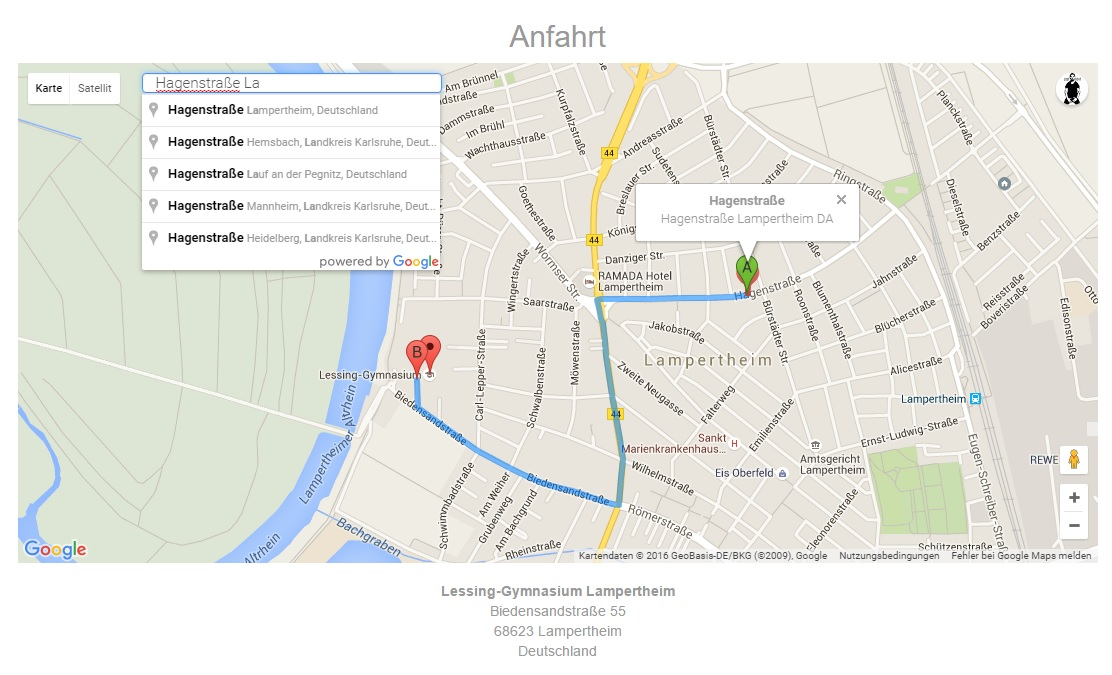
\includegraphics[scale=0.5]{img/googleMaps.jpg}}
	\caption{Anfahrtbeschreibung mit Google Maps}
	\label{fig:googleMaps}
\end{figure}

Auf dem Bild ist nicht nur der Standort der Schule vermerkt, sondern darüberhinaus kann der User über ein Eingabefeld links oben seine Abfahrtsadresse eingeben, sodass die optimale Route auf der Karte angezeigt wird. Des Weiteren wurde mit Hilfe der Autocomplete Funktion der Google Maps API eine automatische Vervollständigung der Adresse bei Eingabe in das Adressfeld implementiert, wie auf dem Screenshot zu sehen ist.
\par
Verwirklicht wurde die Einbindung, indem zuerst



\section{Einbindung von Social Buttons mittels des Heise Plugins}
\label{Einbindung von Social Buttons mittels des Heise Plugins}



\chapter{Client-Server-Kommunikation}
\label{Client-Server-Kommunikation}

\section{Anmeldefunktion per AJAX-Calls}
\label{Anmeldefunktion per AJAX-Calls}

\subsection{Bereitstellung eines REST-Service mit node.js}
\label{Bereitstellung eines REST-Service mit node.js}

\subsection{Konsumieren der Daten im Frontent mit AJAX-Calls}
\label{Konsumieren der Daten im Frontent mit AJAX-Calls}